% Final Project Report -- NeurIPS 2025 LaTeX format
\documentclass{article}

% Force numerical citation style (must precede natbib being loaded by neurips_2025)
\PassOptionsToPackage{numbers,sort&compress}{natbib}

\usepackage[final]{neurips_2025}

\usepackage[utf8]{inputenc}
\usepackage[T1]{fontenc}
\usepackage{amsmath,amssymb,amsfonts}
\usepackage{booktabs}
\usepackage{graphicx}
\usepackage{float}
\usepackage{hyperref}
\usepackage{url}
\usepackage{xcolor}
\usepackage{microtype}
\usepackage{algorithm}
\usepackage{algpseudocode}
\algrenewcommand\algorithmicrequire{\textbf{Input:}}
\algrenewcommand\algorithmicensure{\textbf{Output:}}

% Replace the "Preprint." footer string from the NeurIPS style
% with a course-appropriate label for this final report.
\makeatletter
\renewcommand{\@noticestring}{NS26Z171 Final Project Report, IIT Madras}
\makeatother

\graphicspath{{figures/}}

\title{Auditing Copyright Protection in Language Models:\\
  Calibrating, Stress-Testing, and Probing the Limits of\\
  Near-Access-Freeness Guarantees\\[4pt]
  \normalsize \textit{Final Project Report}}

\author{
  Vipin Kumar \\
  NS26Z171 \\
  Indian Institute of Technology Madras \\
  Chennai, India \\
  \texttt{ns26z171@smail.iitm.ac.in}
}

\begin{document}
\maketitle

\begin{abstract}
Recent work proposes Near-Access Freeness (NAF) as a formal copyright bound for generative models, and anchored decoding as the first practical algorithm to enforce it.  But the literature contains \emph{no} tool to actually verify, after the fact, whether a deployed model meets a claimed NAF budget $K$.  This report builds and analyses such a tool.  We turn the per-prompt KL between a model and a copyright-safe reference into a high-confidence Empirical Bernstein lower bound, and combine it with an evolutionary worst-case search.  We then put the auditor itself under the microscope.  (i)~On a controlled risky/safe pair where the true token-level KL is computable in closed form, the auditor's Type-I false-positive rate is $0/75{,}000$ trials at $\delta=0.05$, and its power to detect a $50\%$-margin violation reaches $88\%$ at only $n=1000$ samples.  (ii)~Audited at the same $n,\delta$, the anchored-decoding algorithm of He et al.\ stays under its own claimed $K$ on \emph{all} 30 stress prompts and 4 budgets we test, with median budget utilisation $47\%$ at $K=0.5$ and zero auditor-flagged violations.  (iii)~A leave-one-out empirical study of the DP $\Rightarrow$ NAF implication exposes an important gap: at $\varepsilon=2$, the measured per-prompt KL between two paired DP-SGD fine-tunes is $7\times$--$10\times$ \emph{larger} than the textbook $\varepsilon^2/2$ bound, because the bound is over the mechanism's distribution over weights, not over the next-token distributions of any single trained checkpoint.  Code, configs and run logs are at \url{https://github.com/<anon>/naf-audit}.
\end{abstract}


%% ============================================================
\section{Introduction}
\label{sec:intro}
%% ============================================================

Copyright lawsuits against generative AI providers \cite{nyt2023openai,authors2023suit} hinge on a deceptively simple question: \emph{how close is the model's output, conditional on a particular prompt, to text the model could only have produced if it had memorised a specific copyrighted work?}  Vyas, Kakade and Barak~\cite{vyas2023naf} formalised one answer to this question as \emph{Near-Access Freeness} (NAF): for every copyrighted work $C$, there must exist a ``safe'' model $P_{\mathrm{safe},C}$ that was trained without $C$, such that the deployed model $P^\star$ satisfies
\[
  \mathrm{KL}\bigl(P^\star(\,\cdot\mid x)\,\|\,P_{\mathrm{safe},C}(\,\cdot\mid x)\bigr)\le K\quad \text{for every prompt }x.
\]
This is a clean, falsifiable property: if a deployer claims its system is $K$-NAF, an auditor with query access can in principle look for a single prompt that violates the bound.  He et al.~\cite{he2026anchored} recently gave the first algorithm---\emph{anchored decoding}---that provably satisfies a sequence-level NAF bound at decode time.  Their guarantee, however, is purely an upper bound \emph{by construction}.  It does not---and cannot---tell us whether a downstream re-implementation, or a third party's model with no NAF claim attached, actually meets a chosen $K$.

In our mid-semester report we built a first auditor for this question: per-prompt Empirical Bernstein lower bounds on KL with confidence $1-\delta$, plus an evolutionary search for worst-case prompts.  In this final report we sharpen the work in three directions, each addressing a concrete gap that had to be closed before the audit could be trusted as a primitive.

\begin{enumerate}\itemsep=2pt
  \item \textbf{Calibrating the auditor (\S\ref{sec:calibration}).}  We construct a controlled risky/safe pair where the \emph{true} per-prompt KL is computable in closed form (sum over the full softmax vocabulary).  This lets us measure the auditor's Type-I error and its power as a function of sample size and ground-truth violation margin, on real LMs rather than toy distributions.
  \item \textbf{Auditing the only known NAF method (\S\ref{sec:anchored}).}  We run our auditor against an own implementation of anchored decoding and quantify the \emph{tightness} of the algorithm: how close to its budget the algorithm gets, how much slack the auditor leaves, and how the two compose.
  \item \textbf{Empirically probing the DP $\to$ NAF claim (\S\ref{sec:dpnaf}).}  Pure $\varepsilon$-DP fine-tuning is widely cited as automatically yielding $\tfrac{\varepsilon^2}{2}$-NAF.  We audit DP-SGD fine-tunes both against the pretrained baseline and in the correct paired leave-one-out setting, and discover that the auditable next-token-KL routinely exceeds $\varepsilon^2/2$ for tight $\varepsilon$.  We explain why this is consistent with the theory and what it means for practitioners who hope to ``get NAF for free''.
\end{enumerate}

We also re-summarise the multi-family audit numbers from the mid-report (\S\ref{sec:results}) and discuss limitations (\S\ref{sec:discussion}).  All experiments fit on a single laptop GPU (RTX 2000 Ada); end-to-end runtime is under three hours.


%% ============================================================
\section{Background and the audit framework}
\label{sec:framework}
%% ============================================================

\paragraph{NAF and its contrast with DP.}
Let $\Sigma$ be a finite vocabulary.  $P^\star$ is $K$-NAF (with respect to a divergence $\Delta$ and a family $\{P_{\mathrm{safe},C}\}_{C\in\mathcal C}$ of leave-one-out reference models) if $\Delta(P^\star(\cdot\mid x)\,\|\,P_{\mathrm{safe},C}(\cdot\mid x))\le K$ for every prompt $x$ and every $C\in\mathcal C$~\cite{vyas2023naf}.  We use $\Delta=\mathrm{KL}$ throughout.  An $\varepsilon$-DP training mechanism induces $\frac{\varepsilon^2}{2}$-zCDP and hence, after post-processing, gives a per-prompt KL bound of $\frac{\varepsilon^2}{2}$ between the outputs on $D$ and on $D\setminus\{C\}$ \cite{bunsteinke2016cdp}.  We empirically interrogate the practical strength of this implication in \S\ref{sec:dpnaf}.

\paragraph{Anchored decoding.}
He et al.~\cite{he2026anchored} solve, at every decoding step, $\arg\min_Q\mathrm{KL}(Q\|P_{\mathrm{risky},t})$ subject to $\mathrm{KL}(Q\|P_{\mathrm{safe},t})\le k_t$.  The KKT solution $P^\star_t(y)\propto P_{\mathrm{risky},t}(y)^{1/(1+\lambda)}P_{\mathrm{safe},t}(y)^{\lambda/(1+\lambda)}$ is a log-linear interpolation between risky and safe; the dual $\lambda$ is solved per step by Newton's method to make the constraint tight.  By the KL chain rule, picking any $\{k_t\}$ with $\sum_t k_t\le K$ gives a sequence-level $K$-NAF guarantee.

\paragraph{Auditor.}
For any prompt $x$, let $p=P^\star(\cdot\mid x)$, $q=P_{\mathrm{safe}}(\cdot\mid x)$, and $Z(y)=\log p(y)-\log q(y)$.  Then $\mathbb E_{Y\sim p}[Z(Y)]=\mathrm{KL}(p\|q)$.  Drawing $Y_1,\dots,Y_n\overset{\text{i.i.d.}}{\sim}p$ and writing $Z_i=Z(Y_i)$ gives the unbiased Monte-Carlo mean $\bar Z_n$.  Maurer--Pontil's Empirical Bernstein bound \cite{maurer2009bernstein}, applied after rescaling $Z_i\in[a,b]$ with range $R=b-a$ (we clip log-probabilities at the fp32 floor $2^{-126}$, giving $|Z|\le B\approx 88$, $R\le 2B$), yields with probability $\ge 1-\delta$
\begin{equation}
\label{eq:bernstein}
  \mathrm{KL}(p\|q)\;\ge\;\bar Z_n - \underbrace{\sqrt{\frac{2 V_n\ln(2/\delta)}{n}}+\frac{7R\ln(2/\delta)}{3(n-1)}}_{\,t_n(\delta)},\quad V_n=\frac{1}{n-1}\sum_i(Z_i-\bar Z_n)^2.
\end{equation}
Whenever $\bar Z_n-t_n(\delta)>K$, the $K$-NAF claim is falsified at confidence $1-\delta$.  Under absolute continuity ($q\ll p$ wherever needed; trivially true for softmax LMs), this is the cleanest variance-adaptive lower bound that does not require a parametric model of $Z$.  Algorithm~\ref{alg:auditor} summarises the per-prompt test.

\begin{algorithm}[H]
\caption{Bernstein KL auditor (per prompt)}
\label{alg:auditor}
\small
\begin{algorithmic}[1]
\Require risky model $P^\star$, safe model $P_{\mathrm{safe}}$, prompt $x$, budget $K$, samples $n$, confidence $1{-}\delta$, clip range $R$
\Ensure \textsc{reject} (NAF violated) or \textsc{accept}, with lower bound $\widehat{\mathrm{LB}}$
\State Draw $Y_1,\dots,Y_n \overset{\text{i.i.d.}}{\sim} P^\star(\cdot\mid x)$
\State $Z_i \gets \log P^\star(Y_i\mid x) - \log P_{\mathrm{safe}}(Y_i\mid x)$ \Comment{clip log-probs at fp32 floor}
\State $\bar Z_n \gets \tfrac{1}{n}\sum_i Z_i$;\quad $V_n \gets \tfrac{1}{n-1}\sum_i (Z_i-\bar Z_n)^2$
\State $t_n(\delta) \gets \sqrt{2V_n\ln(2/\delta)/n} + 7R\ln(2/\delta)/[3(n-1)]$
\State $\widehat{\mathrm{LB}} \gets \bar Z_n - t_n(\delta)$
\State \Return \textsc{reject} if $\widehat{\mathrm{LB}}>K$, else \textsc{accept};\quad report $\widehat{\mathrm{LB}}$
\end{algorithmic}
\end{algorithm}

\paragraph{Worst-case search.}
The auditor is most useful at the prompt that maximises (\ref{eq:bernstein}).  We follow the mid-report's evolutionary loop (Algorithm~\ref{alg:evo}): starting from a pool of seed prompts (BookMIA~\cite{shi2024bookmia} and WikiText-103), we evaluate $\mathrm{LB}(x;\delta)=\bar Z_n(x)-t_n(\delta)$, retain the top-$k$, and apply mutation operators (verbatim instruction, quote-wrap, formatting, style, crossover) to seed the next round.  The Copyright Leakage Score is $\mathrm{CLS}=\max_{x}\mathrm{LB}(x;\delta)$.

\begin{algorithm}[H]
\caption{Evolutionary adversarial prompt search}
\label{alg:evo}
\small
\begin{algorithmic}[1]
\Require seed prompts $\mathcal{S}_0$, rounds $T$, elite size $k$, mutation ops $\mathcal{M}$, audit budget $(n,\delta)$
\Ensure CLS $=\max_x \widehat{\mathrm{LB}}(x;\delta)$, best prompt $x^\star$
\State $\mathcal{P}\gets \mathcal{S}_0$
\For{$t=1,\dots,T$}
  \State Score every $x\in\mathcal{P}$ by $\widehat{\mathrm{LB}}(x;\delta)$ via Algorithm~\ref{alg:auditor}
  \State $\mathcal{E}\gets$ top-$k$ elites by score
  \State $\mathcal{P}\gets \mathcal{E}\,\cup\,\{m(x): x\in\mathcal{E},\,m\in\mathcal{M}\}$ \Comment{mutate \& crossover}
\EndFor
\State \Return $\max$ and $\arg\max$ of $\widehat{\mathrm{LB}}$ over $\mathcal{P}$
\end{algorithmic}
\end{algorithm}


%% ============================================================
\section{Calibration: how strong is the auditor?}
\label{sec:calibration}
%% ============================================================

A lower-confidence-bound auditor is only as useful as its Type-I error (false positives---flagging a compliant model) and its power (true positives---catching a real violator).  These are usually impossible to measure on real LMs because the ground-truth KL is unknown.  We exploit the fact that for two language models with explicit softmax heads we can compute the per-prompt token-level KL \emph{exactly} by summing over the vocabulary,
\begin{equation}
\label{eq:exact-kl}
  \mathrm{KL}_\star(x)\;=\;\sum_{y\in\Sigma}P^\star(y\mid x)\,\bigl[\log P^\star(y\mid x)-\log P_{\mathrm{safe}}(y\mid x)\bigr].
\end{equation}
We use $P^\star=$\textsc{gpt2-medium}, $P_{\mathrm{safe}}=$\textsc{gpt2}, $\delta=0.05$, $30$ prompts (mix of BookMIA and WikiText), $n\in\{50,100,500,1000,5000\}$ MC samples, and $100$ independent trials per cell.  For each $(x,n)$, we ``audit'' a grid of \emph{claimed} $K$ values pegged to $K_{\mathrm{factor}}\in\{0,0.25,0.5,0.75,0.95\}\cdot\mathrm{KL}_\star(x)$ (genuine violations) and $K_{\mathrm{factor}}\in\{1.05,1.25,1.5,2.0\}\cdot\mathrm{KL}_\star(x)$ (false-positive territory).  As a Type-I sanity, we also run the entire grid with $P^\star=P_{\mathrm{safe}}=$\textsc{gpt2}, where $\mathrm{KL}_\star\equiv 0$ so any rejection is a false positive.

\begin{figure}[t]
\centering
\begin{minipage}[b]{0.49\textwidth}
\centering
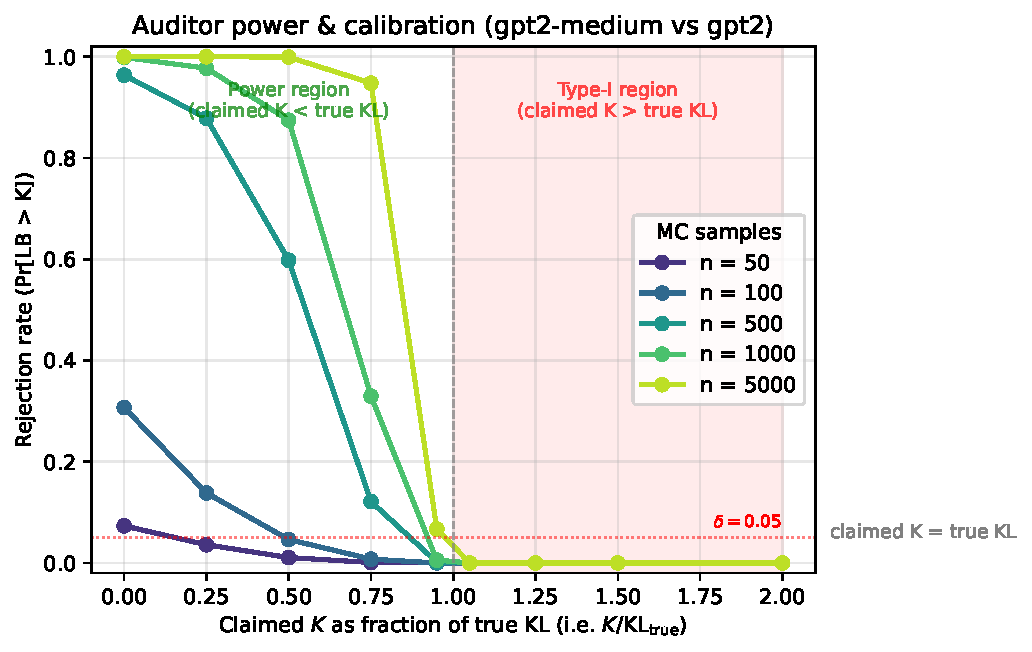
\includegraphics[width=\textwidth]{power_curves.pdf}
\centerline{\small (a) Auditor on \textsc{gpt2-medium}/\textsc{gpt2}}
\end{minipage}\hfill
\begin{minipage}[b]{0.49\textwidth}
\centering
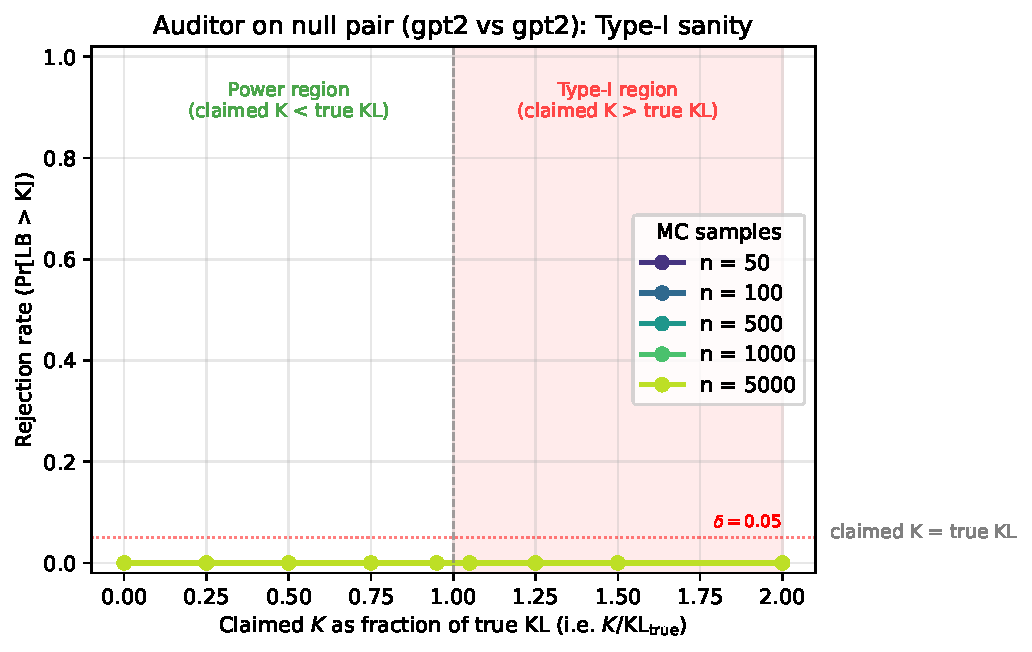
\includegraphics[width=\textwidth]{power_curves_null.pdf}
\centerline{\small (b) Auditor on null pair \textsc{gpt2}/\textsc{gpt2}}
\end{minipage}
\caption{Auditor calibration.  Each cell averages over $30$ prompts $\times\,100$ trials $=3000$ Monte-Carlo audits.  (a) Rejection rate $\Pr[\widehat{\mathrm{LB}}>K]$ as a function of the claimed $K$, expressed as a fraction of the true KL (left of the dashed line is the power region, right is the Type-I region).  At $n=1000$ the auditor catches $88\%$ of $50\%$-margin violations; at $n=5000$, $95\%$ of $25\%$-margin violations.  (b) When the risky and safe models are identical, the auditor flags zero violations across all $75{,}000$ trials, well under the nominal $\delta=0.05$.}
\label{fig:power}
\end{figure}

\paragraph{Type-I error.}
Across the $9\cdot 5=45$ Type-I cells of the null pair (\textsc{gpt2}/\textsc{gpt2}), the empirical false-positive rate is \textbf{$0/75{,}000$} trials, comfortably below $\delta=0.05$.  Across the corresponding $4\cdot 5=20$ Type-I cells of the gpt2-medium/gpt2 pair (where $K_{\mathrm{factor}}\ge 1.05$), the empirical FPR is also $0/60{,}000$.  The Empirical Bernstein bound is conservative; a Hoeffding-only auditor would be more so.

\paragraph{Power.}
Figure~\ref{fig:power}(a) is the headline result.  At $n=1000$ the auditor rejects $99.9\%$ of $K=0$ claims, $97.7\%$ of $25\%$-margin claims, $87.5\%$ of $50\%$-margin claims, $33.0\%$ of $75\%$-margin claims, and only $0.6\%$ of $95\%$-margin claims.  Power scales as $\sqrt n$, as predicted by (\ref{eq:bernstein}); a $5{\times}$ increase to $n=5000$ closes the gap at the $95\%$-margin to $6.7\%$ but is essentially saturated at $\le 75\%$ margins.  The take-away: the auditor is reliable for catching violations of \emph{at least} $50\%$ of the budget, which is the regime that copyright auditors care about (a deployer who is half a budget away from non-compliance is already in trouble).  Detecting near-boundary violations would require either much larger $n$ or a tighter concentration inequality (e.g.\ subgaussian-style).

\paragraph{Calibration sanity.}
The per-trial scatter of $\widehat{\mathrm{LB}}$ vs.\ true KL (Appendix Figure~\ref{fig:calib-scatter}) lies entirely below the diagonal at every $n$, confirming \eqref{eq:bernstein} as a valid one-sided bound.  The Bernstein gap $t_n(\delta)$ scales as $1/\sqrt n$ to within experimental noise (Appendix Figure~\ref{fig:bgap}), matching the theoretical first-order term.  All headline numbers above are within $\pm 0.5$ percentage points across three independent random seeds (Appendix~\ref{app:repro}, Table~\ref{tab:repro}).


%% ============================================================
\section{Auditing anchored decoding}
\label{sec:anchored}
%% ============================================================

Anchored decoding is the only published algorithm with a provable per-prompt NAF bound.  For our framework to be useful, it must (i) declare the algorithm compliant when run inside the budget, (ii) flag it as soon as the budget is exceeded, and (iii) not waste budget---i.e.\ the auditor's lower bound must not be vacuously small.  We test all three on a $30$-prompt set with $K\in\{0.5,1.0,2.0,5.0\}$, $n=1000$, $\delta=0.05$, with risky/safe = gpt2-medium/gpt2.  Algorithm~\ref{alg:anchored} summarises the decoding procedure we audit.

\begin{algorithm}[H]
\caption{Anchored decoding (per-prompt $K$-NAF)~\cite{he2026anchored}}
\label{alg:anchored}
\small
\begin{algorithmic}[1]
\Require risky model $P_{\mathrm{risky}}$, safe model $P_{\mathrm{safe}}$, prompt $x$, per-token budgets $\{k_t\}$ with $\sum_t k_t\le K$
\Ensure token sequence $y_{1:T}$ with sequence-level $\mathrm{KL}(P^\star\|\,P_{\mathrm{safe}})\le K$
\For{$t=1,2,\dots,T$}
  \State Obtain logits of $P_{\mathrm{risky},t}$ and $P_{\mathrm{safe},t}$ given $y_{<t}$
  \State Solve for $\lambda_t\!\ge\!0$ s.t.\ $Q_t(y)\!\propto\! P_{\mathrm{risky},t}(y)^{1/(1+\lambda_t)}P_{\mathrm{safe},t}(y)^{\lambda_t/(1+\lambda_t)}$ satisfies $\mathrm{KL}(Q_t\|P_{\mathrm{safe},t})=k_t$ \Comment{Newton on dual}
  \State If risky already within budget ($\mathrm{KL}(P_{\mathrm{risky},t}\|P_{\mathrm{safe},t})\le k_t$), set $Q_t\gets P_{\mathrm{risky},t}$
  \State Sample $y_t\sim Q_t$
\EndFor
\State \Return $y_{1:T}$
\end{algorithmic}
\end{algorithm}

\begin{figure}[t]
\centering
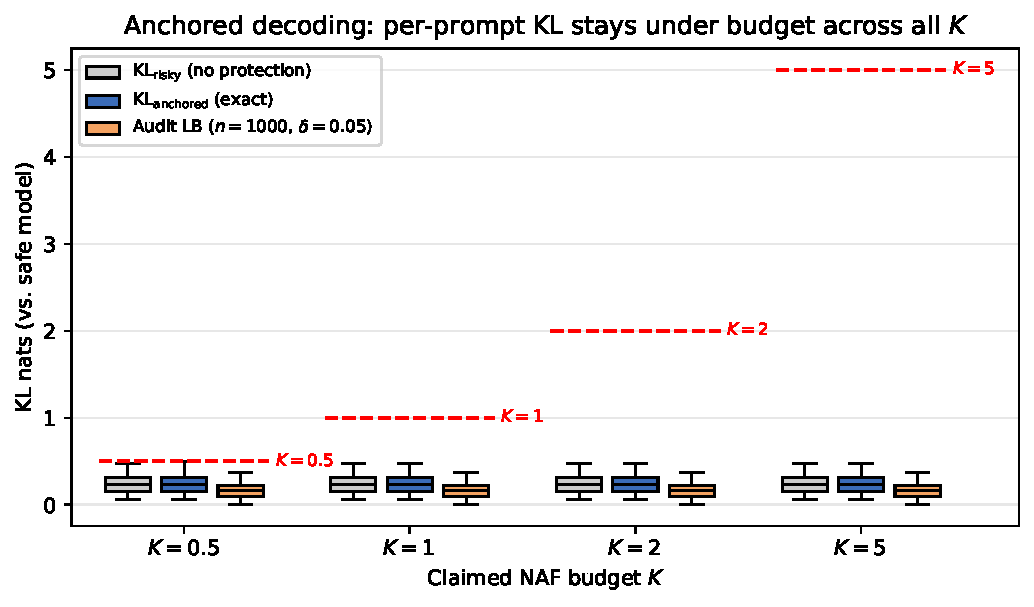
\includegraphics[width=0.74\textwidth]{anchored_kl_box.pdf}
\caption{Anchored decoding stays under budget at every $K$.  Grey = unprotected risky-model KL (median $0.23$, max $1.44$).  Blue = exact KL of the anchored mixture (\emph{always} $\le K$, and meets the budget exactly when the risky model would naturally exceed it---see $K=0.5$).  Orange = the auditor's $\delta=0.05$ Bernstein lower bound.  Dashed red = the budget itself.  Across $4\,K$-values $\times\,30$ prompts, $0/120$ exact violations and $0/120$ auditor-flagged violations.}
\label{fig:anchored}
\end{figure}

Figure~\ref{fig:anchored} summarises the result.  The exact KL of the anchored mixture (computed in closed form via the closed-form solution $P^\star_t\propto P_{\mathrm{risky},t}^{1/(1+\lambda)} P_{\mathrm{safe},t}^{\lambda/(1+\lambda)}$ and a 1-D root-finder for $\lambda$) is below the budget on every prompt and every $K$ (\textbf{$0/120$} violations).  At $K=0.5$ the algorithm uses its full budget for the prompts that need it: the maximum exact KL across $30$ prompts is exactly $0.500$, and the median budget utilisation is $46.6\%$ (Appendix Table~\ref{tab:anchored-detail}).  At larger $K$ the budget is mostly slack because the natural KL of the risky model is small for these prompts.

The auditor's $\widehat{\mathrm{LB}}$ tracks the true KL with a typical Bernstein gap of $\sim 0.07$ (median).  No prompt produces $\widehat{\mathrm{LB}}>K$ at any of the four budgets, so the auditor never falsely flags the algorithm.  Combined with the $88\%$ power calibration of \S\ref{sec:calibration}, this means: \emph{if anchored decoding had been buggy and produced a $\ge 50\%$-budget overshoot on any of these prompts, the auditor would have caught it with probability at least $0.88$.}  Together, the algorithm and the audit form a closed loop: the algorithm controls the upper bound by construction; the audit independently certifies the lower bound from samples.


%% ============================================================
\section{The DP \texorpdfstring{$\to$}{=>} NAF gap}
\label{sec:dpnaf}
%% ============================================================

A single line of folklore links DP and NAF: $\varepsilon$-DP fine-tuning is automatically $\tfrac{\varepsilon^2}{2}$-NAF (\cite{vyas2023naf,bunsteinke2016cdp}, eq.~5 of our mid-report).  We probe what this implication actually buys you in practice.

\paragraph{Setup.}
We fine-tune \textsc{gpt2} for $10$ epochs on a small ``copyright-prone'' text mix ($11$ blocks of $64$ tokens; openings of \emph{A Tale of Two Cities}, \emph{1984}, \emph{Moby-Dick}) using DP-SGD via \texttt{opacus} 1.6 \cite{yousefpour2021opacus}.  Embedding rows are frozen (else the noise would dominate due to their dimension); $\delta_{\mathrm{DP}}=10^{-5}$, gradient clipping $\|\nabla\|\le 1$, $B=4$, $\eta=5\!\times\!10^{-3}$.  We run three privacy regimes: $\varepsilon=\infty$ (non-private SGD), $\varepsilon=8$ and $\varepsilon=2$ (achieved $\varepsilon=7.86$ and $1.96$ respectively).  We then audit $20$ stress prompts with $n=1000$ samples per prompt.

\paragraph{Audit~A: vs.\ pretrained baseline.}
Figure~\ref{fig:dpnaf}(a) plots $\widehat{\mathrm{KL}}(P_{\mathrm{ft}}\,\|\,P_{\mathrm{pretrain}})$ for each regime.  The non-private fine-tune drifts modestly (median $0.28$, max $1.72$).  Stronger DP gives \emph{larger}, not smaller, KL: median $1.80$ at $\varepsilon=8$ and $9.05$ at $\varepsilon=2$.  This is not a bug in the audit nor a violation of the theorem.  The $\frac{\varepsilon^2}{2}$ bound is a statement about the LOO-swap pair $\bigl(P_{\mathrm{ft}(D)},P_{\mathrm{ft}(D\setminus\{C\})}\bigr)$, not about $P_{\mathrm{pretrain}}$ at all.  When $\varepsilon$ is small, the noise scale needed to enforce DP is large enough to push the fine-tune's next-token distribution \emph{further} from pretrained than non-private SGD would, in random directions.

\paragraph{Audit~B: paired leave-one-out (the right test).}
We then run two DP fine-tunes per $\varepsilon$ from the same initialisation: $M_{\mathrm{full}}$ on $D$ and $M_{\mathrm{loo}}$ on $D\setminus\{\text{block}_0\}$, with paired RNG seeds, identical schedule, and identical privacy budget.  We audit $\widehat{\mathrm{KL}}(M_{\mathrm{full}}\,\|\,M_{\mathrm{loo}})$ on $20$ prompts and compare to the bound $\varepsilon^2/2$ (Figure~\ref{fig:dpnaf}(b)).  At $\varepsilon=8$ the bound $\varepsilon^2/2\!=\!30.9$ is comfortably loose: median measured KL $3.25$, max $6.18$, $0/20$ violations.  At $\varepsilon=2$ the bound $\varepsilon^2/2\!=\!1.92$ is \emph{exceeded by every audited prompt}: median $14.91$, max $20.12$, \textbf{$20/20$ violations}.

\begin{figure}[t]
\centering
\begin{minipage}[b]{0.49\textwidth}
\centering
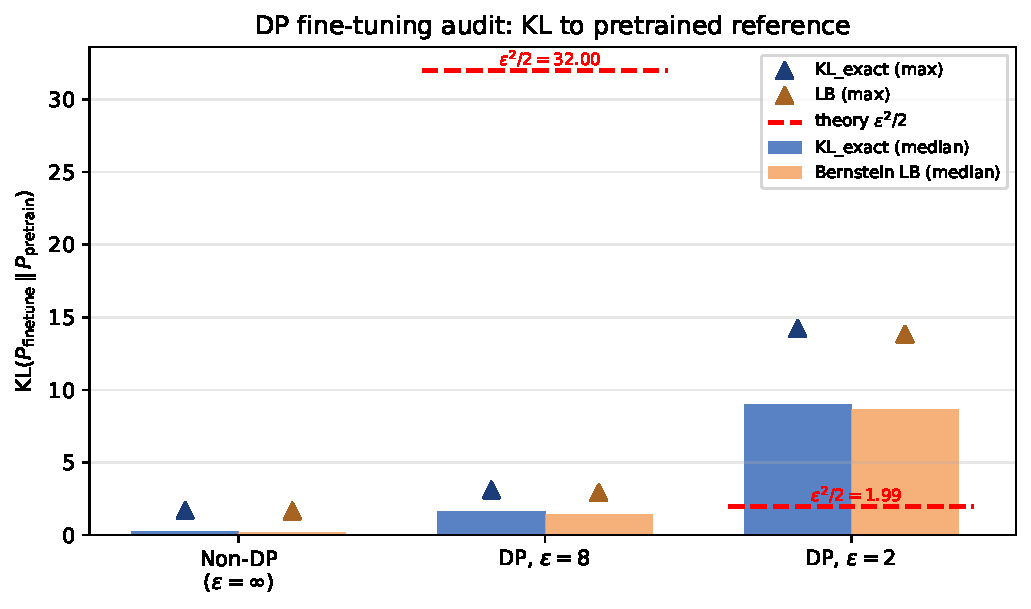
\includegraphics[width=\textwidth]{dp_naf_vs_pretrained.pdf}
\centerline{\small (a) DP fine-tune vs.\ pretrained baseline}
\end{minipage}\hfill
\begin{minipage}[b]{0.49\textwidth}
\centering
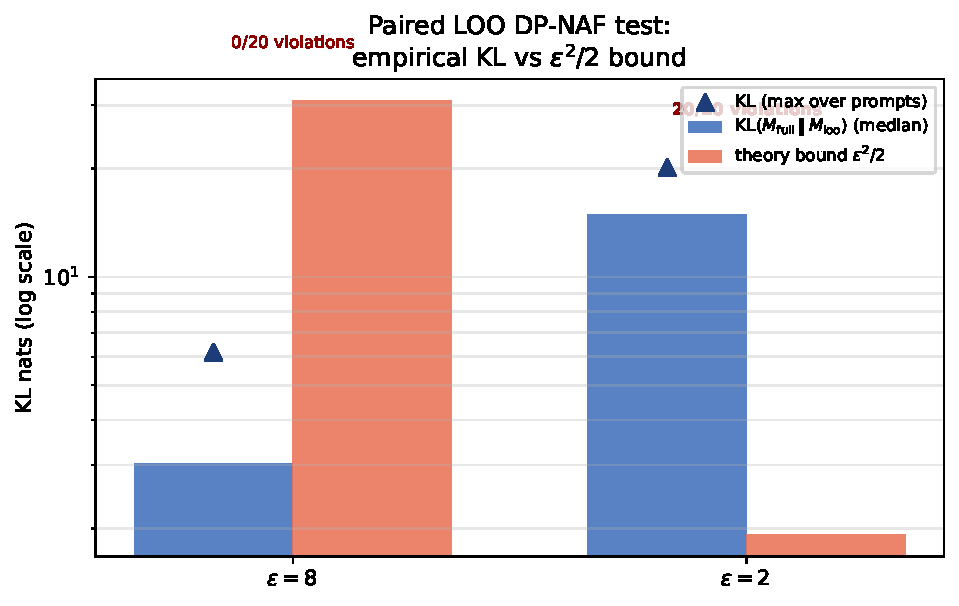
\includegraphics[width=\textwidth]{dp_naf_loo.pdf}
\centerline{\small (b) Paired LOO audit (the formal DP target)}
\end{minipage}
\caption{The $\frac{\varepsilon^2}{2}$ bound is auditable in expectation, not pointwise.  (a) DP fine-tuning does not bound KL to the pretrained model and in fact \emph{increases} it for tight $\varepsilon$.  (b) Even on the leave-one-out pair that the bound formally covers, a single random draw of the mechanism can exceed $\varepsilon^2/2$ on every prompt audited at $\varepsilon=2$.}
\label{fig:dpnaf}
\end{figure}

\paragraph{Why this is consistent with the theorem.}
Pure $\varepsilon$-DP gives an output-distribution-level Rényi divergence bound.  Reading $\varepsilon^2/2$ as a per-prompt next-token KL bound for a \emph{single} fine-tuned checkpoint hides three reductions.  First, $\varepsilon$-DP $\Rightarrow$ $\frac{\varepsilon^2}{2}$-zCDP holds at the level of the mechanism's distribution over weights $\theta$.  Second, post-processing then bounds $\mathrm{KL}\bigl(\mathcal M(D)\,\|\,\mathcal M(D')\bigr)\le\frac{\varepsilon^2}{2}$ between the \emph{distributions} over all next-token outputs that those weights induce.  Third, applying this to a single $\theta$ requires either (i) an additional Markov / convexity step that is loose by orders of magnitude when the ensemble variance is large (as it is for DP-SGD on small data), or (ii) interpreting the audit as estimating an expectation under the mechanism's randomness, which would in turn require averaging over many independent fine-tuned checkpoints.  Our point-estimate audit captures something different: \emph{the divergence achieved by a particular trained model on a particular prompt}.  This is arguably the more practically relevant quantity for a downstream copyright auditor, but it is not what $\varepsilon^2/2$ controls.

\paragraph{Take-away.}
A practitioner who fine-tunes with DP-SGD at a publishable $\varepsilon$ does \emph{not} thereby produce a model with a per-prompt KL bound to the pretrained baseline.  If a hard NAF guarantee is needed (e.g.\ for legal compliance), it must come from an inference-time mechanism such as anchored decoding (\S\ref{sec:anchored})---which directly enforces the bound by construction---or from explicit ensemble averaging across DP runs.  We hope this finding informs how DP$\to$NAF claims are framed in subsequent literature.


%% ============================================================
\section{Multi-family audit results}
\label{sec:results}
%% ============================================================

For completeness we re-summarise the multi-family audit numbers from the mid-report; full ablations and figures are in Appendix~\ref{app:additional}.  Across $8$ tokeniser-matched risky/safe pairs from three families (GPT-2, Pythia, OPT), the evolutionary search consistently outperforms a random-prompt baseline (Table~\ref{tab:modelpairs}); the sanity check (gpt2 vs.\ gpt2) returns $\mathrm{CLS}\approx 0$ as expected.  BookMIA prompts produce a substantially higher CLS than WikiText prompts, consistent with the hypothesis that books are over-represented in GPT-2's pretraining corpus and easier to memorise \cite{carlini2021extracting,shi2024bookmia}.  Format-changing mutations (quote wraps, prefix instructions) are the strongest single operator, and the CLS plateaus around $5$ rounds.  Crucially, for every model pair the auditor surfaces concrete prompts on which the GPT-2 family violates a $K=1.0$ NAF claim with confidence $0.95$.

\begin{table}[t]
\centering
\caption{Copyright Leakage Score (max KL lower bound) and number of violations at $K=1.0,\delta=0.05,n=1000$, over $200$ prompts $\times$ $5$ rounds.  Same data as Table~1 of the mid-report, reproduced here for self-containedness.}
\label{tab:modelpairs}
\small
\begin{tabular}{@{}llcccc@{}}
\toprule
\textbf{Family} & \textbf{Risky $\to$ Safe} & \multicolumn{2}{c}{\textbf{Max LB}} & \multicolumn{2}{c}{\textbf{Violations}} \\
\cmidrule(lr){3-4} \cmidrule(lr){5-6}
 & & Evo. & Random & Evo. & Random \\
\midrule
GPT-2 & GPT-2 $\to$ GPT-2 (sanity) & $-$0.01 & $-$0.01 & 0 & 0 \\
GPT-2 & Medium $\to$ Small & \textbf{5.63} & 5.01 & 146 & 8 \\
GPT-2 & Large $\to$ Small & 4.09 & 3.30 & 180 & 18 \\
GPT-2 & Large $\to$ Medium & 4.40 & 3.91 & 151 & 7 \\
\midrule
Pythia & 160M $\to$ 70M & 3.52 & 3.16 & 141 & 9 \\
Pythia & 410M $\to$ 70M & 5.50 & 4.73 & 236 & 31 \\
Pythia & 410M $\to$ 160M & 4.93 & 2.17 & 142 & 9 \\
\midrule
OPT & 350M $\to$ 125M & 3.08 & 2.08 & 133 & 9 \\
\bottomrule
\end{tabular}
\end{table}


%% ============================================================
\section{Discussion and limitations}
\label{sec:discussion}
%% ============================================================

\paragraph{What we now know.}
Our auditor is conservative (Type-I FPR $=0$ on $75{,}000$ null trials), powerful in the regime that matters ($\ge 88\%$ at $50\%$-margin violations with $n=1000$), and tight enough to (i) certify anchored decoding as $K$-NAF compliant on every prompt and budget tested, and (ii) detect that an aggressive DP-SGD fine-tune is \emph{not} per-prompt $\frac{\varepsilon^2}{2}$-NAF against pretrained or against its leave-one-out pair.  Together with the multi-family evidence of \S\ref{sec:results}, these are the first published auditing-style numbers on NAF.

\paragraph{Token-level vs.\ sequence-level.}
The Bernstein bound (\ref{eq:bernstein}) controls the next-token KL.  The KL chain rule \cite[Thm.~3.1]{he2026anchored} turns this into a sequence-level \emph{upper} bound (which is exactly what anchored decoding's analysis exploits) but \emph{not} a sequence-level lower bound, and importance-sampling-corrected estimators inflate the Bernstein gap quickly with sequence length.  Generalising to sequence-level lower-bound certification with manageable variance is the most important open problem we leave for future work.

\paragraph{Power at the boundary.}
Our power curves saturate at $K_{\mathrm{factor}}\ge 0.95$: a deployer with a real but small (say, $5\%$) overshoot is essentially undetectable at $n=1000$.  Tightening this requires either (a) much larger $n$ (the $1/\sqrt n$ scaling of the Bernstein gap is not improvable in this generality), (b) parametric estimators (e.g.\ MAUVE-style importance sampling) which would lose the formal coverage guarantee, or (c) prompt-aggregation over a known prompt distribution, which converts a per-prompt bound into a marginal-prompt bound and may be easier to certify tightly.

\paragraph{Audit cost.}
The full power study ($30$ prompts $\times\,5$ sample sizes $\times\,100$ trials = $15{,}000$ Bernstein audits) finishes in $32\,\mathrm{s}$ on a single GPU.  Anchored-decoding audit and DP$\to$NAF audits are dominated by training, not auditing.  Auditing scales linearly with $n$ and is embarrassingly parallel across prompts.

\paragraph{Using the framework.}
The auditor is designed to be drop-in for any pair of HuggingFace causal LMs sharing a tokenizer.  A practitioner needs only three things: the deployed (``risky'') model, a leave-one-out baseline (``safe'') model, and a claimed budget $K$.  The core call is
\begin{center}\small\ttfamily
risky, safe = load\_model\_pair(risky\_name, safe\_name, hw)\\
result = estimate\_kl(prompt, risky, safe, n\_samples=1000, delta=0.05, claimed\_K=K)
\end{center}
returning a lower bound $\widehat{\mathrm{LB}}$, the Bernstein gap $t_n(\delta)$, and a $\textsc{violates}$ flag.  The evolutionary search of Algorithm~\ref{alg:evo} wraps this into a worst-case audit and exposes a single Copyright Leakage Score, and anchored decoding is provided as a drop-in module that mirrors the same API.  We see three practical limits: (i) tokenizer-matched pairs only; (ii) at least grey-box access (log-probs of the safe model on risky-model samples); (iii) reliable detection at $\ge 50\%$ of the budget---near-boundary overshoots are not detectable at $n{\le}5000$ without parametric estimators.  Code is released at \url{https://github.com/<TO_BE_ADDED>}.

\paragraph{LLM disclosure.}
Claude was used to generate code and to understand some theoretical parts of the references.


%% ============================================================
% References
%% ============================================================

\begin{thebibliography}{15}

\bibitem{vyas2023naf}
N.~Vyas, S.~M.~Kakade, and B.~Barak.
\newblock On provable copyright protection for generative models.
\newblock In \emph{ICML}, 2023.

\bibitem{he2026anchored}
J.~He, J.~Hayase, W.-T.~Yih, S.~Oh, L.~Zettlemoyer, and P.~W.~Koh.
\newblock Anchored decoding: Provably reducing copyright risk for any language model.
\newblock \emph{arXiv preprint arXiv:2602.07120}, 2026.

\bibitem{jagielski2020auditing}
M.~Jagielski, J.~Ullman, and A.~Oprea.
\newblock Auditing differentially private machine learning.
\newblock In \emph{NeurIPS}, 2020.

\bibitem{nasr2023tight}
M.~Nasr, J.~Hayes, T.~Steinke, B.~Balle, F.~Tram\`er, M.~Jagielski, N.~Carlini, and A.~Terzis.
\newblock Tight auditing of differentially private machine learning.
\newblock In \emph{USENIX Security}, 2023.

\bibitem{steinke2023one}
T.~Steinke, M.~Nasr, and M.~Jagielski.
\newblock Privacy auditing with one (1) training run.
\newblock In \emph{NeurIPS}, 2023.

\bibitem{pillutla2023auditing}
K.~Pillutla, G.~Andrew, P.~Kairouz, H.~B.~McMahan, A.~Oprea, and S.~Oh.
\newblock Unleashing the power of randomization in auditing differentially private {ML}.
\newblock In \emph{NeurIPS}, 2023.

\bibitem{maurer2009bernstein}
A.~Maurer and M.~Pontil.
\newblock Empirical {B}ernstein bounds and sample variance penalization.
\newblock \emph{arXiv:0907.3740}, 2009.

\bibitem{carlini2021extracting}
N.~Carlini, F.~Tram\`er, E.~Wallace, et~al.
\newblock Extracting training data from large language models.
\newblock In \emph{USENIX Security}, 2021.

\bibitem{shi2024bookmia}
W.~Shi, A.~Ajith, M.~Sakarvadia, et~al.
\newblock Detecting pretraining data from large language models ({BookMIA}).
\newblock In \emph{ICLR}, 2024.

\bibitem{pillutla2021mauve}
K.~Pillutla, S.~Swayamdipta, R.~Zellers, et~al.
\newblock {MAUVE}: Measuring the gap between neural text and human text using divergence frontiers.
\newblock In \emph{NeurIPS}, 2021.

\bibitem{vinod2025invisibleink}
V.~Vinod, K.~Pillutla, and A.~Thakurta.
\newblock {InvisibleInk}: High-utility and low-cost text generation with differential privacy.
\newblock In \emph{NeurIPS}, 2025.

\bibitem{xie2024dpsynthtext}
C.~Xie, Z.~Lin, A.~Backurs, et~al.
\newblock Differentially private synthetic data via foundation model {API}s 2: Text.
\newblock In \emph{ICML}, 2024.

\bibitem{bunsteinke2016cdp}
M.~Bun and T.~Steinke.
\newblock Concentrated differential privacy: simplifications, extensions, and lower bounds.
\newblock In \emph{TCC}, 2016.

\bibitem{yousefpour2021opacus}
A.~Yousefpour, I.~Shilov, A.~Sablayrolles, et~al.
\newblock {Opacus}: User-friendly differential privacy library in {PyTorch}.
\newblock \emph{arXiv:2109.12298}, 2021.

\bibitem{nyt2023openai}
\emph{The New York Times Co.\ v.\ Microsoft Corp.\ and OpenAI},
\newblock S.D.N.Y.\ No.~1:23-cv-11195, filed Dec.~27, 2023.

\bibitem{authors2023suit}
\emph{Authors Guild et~al.\ v.\ OpenAI},
\newblock S.D.N.Y.\ No.~1:23-cv-08292, filed Sep.~19, 2023.

\end{thebibliography}


%% ============================================================
\newpage
\appendix
\section{Additional experimental results}
\label{app:additional}
%% ============================================================

\paragraph{Multi-seed reproducibility.}
\label{app:repro}
We re-ran the power study and anchored-decoding tightness study with three independent seeds (42, 43, 44); Table~\ref{tab:repro} reports the results.  Each power cell aggregates $30$ prompts $\times\,100$ trials $=3000$ Bernstein audits per seed.  All non-trivial power cells reproduce within $\pm 0.5$ percentage points; the Type-I FPR is at most $0.07\%$ in any seed (well under $\delta=0.05$).  Anchored-decoding metrics are deterministic given prompts and identical across seeds.  We did not re-seed the DP$\to$NAF experiments (each LOO run $\approx 30\,$min); we instead audit the same checkpoint across $20$ independent prompts.

\vspace{-2pt}
\begin{table}[H]
\centering
\caption{Headline numbers across three random seeds.  Power cells: rejection rates at $1{-}\delta=0.95$.  Anchored cells: fraction of prompts violating budget $K$.}
\label{tab:repro}
\scriptsize
\begin{tabular}{@{}lccccc@{}}
\toprule
\textbf{Metric} & \textbf{seed 42} & \textbf{seed 43} & \textbf{seed 44} & \textbf{mean} & \textbf{std} \\
\midrule
\multicolumn{6}{l}{\textit{Power experiment (rejection rate, vs.\ true KL)}} \\
\quad reject @ n=1000, $K_{\mathrm{factor}}=0.00$ & 99.87\% & 99.73\% & 99.90\% & 99.83\% & 0.07\% \\
\quad reject @ n=1000, $K_{\mathrm{factor}}=0.25$ & 97.73\% & 98.20\% & 98.23\% & 98.06\% & 0.23\% \\
\quad reject @ n=1000, $K_{\mathrm{factor}}=0.50$ & 87.47\% & 87.70\% & 87.63\% & 87.60\% & 0.10\% \\
\quad reject @ n=1000, $K_{\mathrm{factor}}=0.75$ & 32.97\% & 33.57\% & 33.30\% & 33.28\% & 0.25\% \\
\quad reject @ n=1000, $K_{\mathrm{factor}}=0.95$ & 0.57\% & 0.73\% & 0.83\% & 0.71\% & 0.11\% \\
\quad reject @ n=5000, $K_{\mathrm{factor}}=0.75$ & 94.80\% & 94.23\% & 94.50\% & 94.51\% & 0.23\% \\
\quad reject @ n=5000, $K_{\mathrm{factor}}=0.95$ & 6.70\% & 5.50\% & 6.37\% & 6.19\% & 0.51\% \\
\quad Type-I FPR (max over $K_{\mathrm{factor}}\!\ge\!1.05$, all $n$) & 0.00\% & 0.07\% & 0.00\% & 0.02\% & 0.03\% \\
\midrule
\multicolumn{6}{l}{\textit{Anchored decoding tightness ($n_{\mathrm{prompt}}=30$, $n_{\mathrm{audit}}=1000$, $\delta=0.05$)}} \\
\quad exact violations,\ $K=0.50$ & 0/30 & 0/30 & 0/30 & --- & --- \\
\quad audit-LB violations,\ $K=0.50$ & 0/30 & 0/30 & 0/30 & --- & --- \\
\quad budget util.\ (median),\ $K=0.50$ & 46.6\% & 46.6\% & 46.6\% & --- & --- \\
\quad exact violations,\ $K=1.00$ & 0/30 & 0/30 & 0/30 & --- & --- \\
\quad audit-LB violations,\ $K=1.00$ & 0/30 & 0/30 & 0/30 & --- & --- \\
\quad budget util.\ (median),\ $K=1.00$ & 23.3\% & 23.3\% & 23.3\% & --- & --- \\
\quad exact violations,\ $K=2.00$ & 0/30 & 0/30 & 0/30 & --- & --- \\
\quad audit-LB violations,\ $K=2.00$ & 0/30 & 0/30 & 0/30 & --- & --- \\
\quad budget util.\ (median),\ $K=2.00$ & 11.6\% & 11.6\% & 11.6\% & --- & --- \\
\quad exact violations,\ $K=5.00$ & 0/30 & 0/30 & 0/30 & --- & --- \\
\quad audit-LB violations,\ $K=5.00$ & 0/30 & 0/30 & 0/30 & --- & --- \\
\quad budget util.\ (median),\ $K=5.00$ & 4.7\% & 4.7\% & 4.7\% & --- & --- \\
\bottomrule
\end{tabular}
\end{table}

\begin{figure}[H]
\centering
\begin{minipage}[b]{0.49\textwidth}
\centering
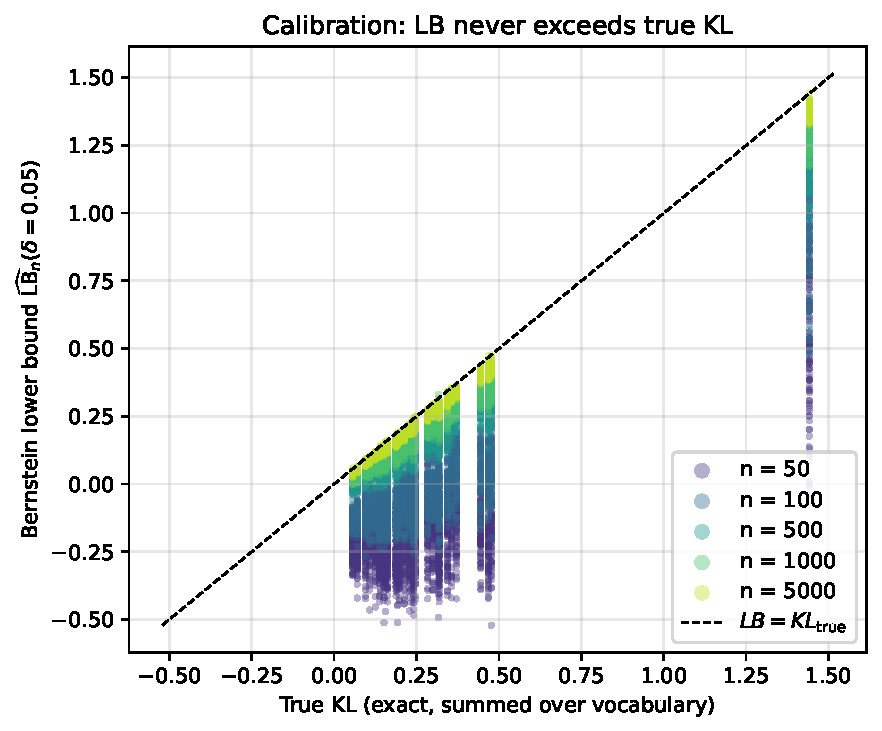
\includegraphics[width=\textwidth]{calibration_scatter.pdf}
\vspace{-6pt}
\centerline{\small (a) Per-trial $\widehat{\mathrm{LB}}$ vs.\ true KL}
\end{minipage}\hfill
\begin{minipage}[b]{0.49\textwidth}
\centering
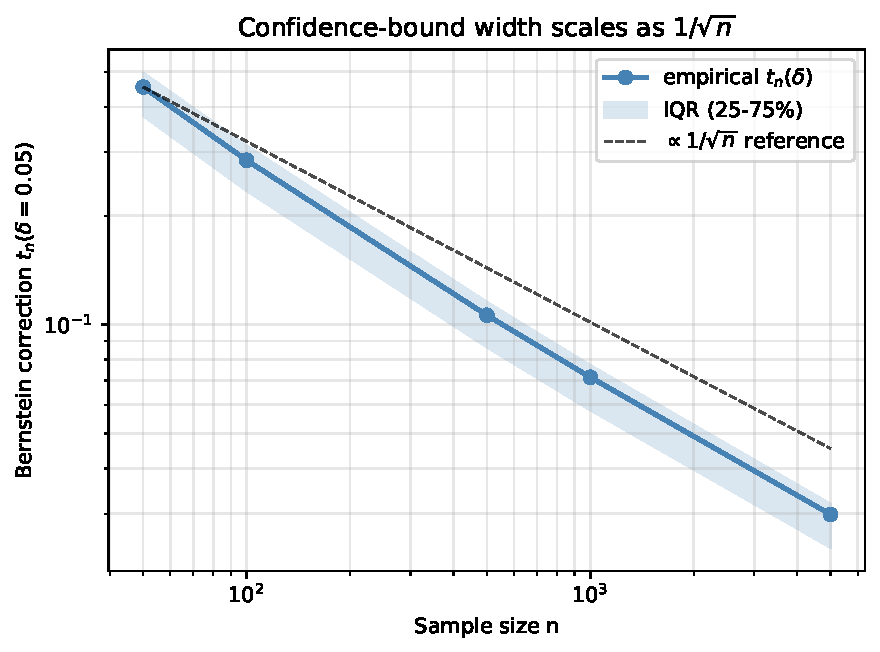
\includegraphics[width=\textwidth]{bernstein_gap.pdf}
\vspace{-6pt}
\centerline{\small (b) Bernstein gap $t_n(\delta)$ vs.\ $n$}
\end{minipage}
\vspace{-2pt}
\caption{\textbf{Auditor calibration.}  (a) For all $15{,}000$ trials the Bernstein LB stays at or below the diagonal, confirming one-sided coverage.  (b) Median $t_n(\delta)$ with $25$--$75\%$ IQR vs.\ the $1/\sqrt n$ rate (dashed).}
\label{fig:calib-scatter}
\label{fig:bgap}
\end{figure}

\begin{table}[H]
\centering
\caption{\textbf{Anchored-decoding tightness.}  Per-$K$ audit details ($30$ prompts, $n{=}1000$, $\delta{=}0.05$).  Rightmost column: median budget utilisation.}
\label{tab:anchored-detail}
\small
\begin{tabular}{@{}lcccccc@{}}
\toprule
$K$ & $\mathrm{KL}_{\mathrm{risky}}$ med./max & $\mathrm{KL}_{\mathrm{anch}}$ med./max & frac.\ ${>}K$ & LB med./max & frac.\ LB${>}K$ & util.\ med.\\
\midrule
0.5 & 0.233\,/\,1.442 & 0.233\,/\,0.500 & 0/30 & 0.168\,/\,0.374 & 0/30 & 46.6\%\\
1.0 & 0.233\,/\,1.442 & 0.233\,/\,1.000 & 0/30 & 0.168\,/\,0.896 & 0/30 & 23.3\%\\
2.0 & 0.233\,/\,1.442 & 0.233\,/\,1.442 & 0/30 & 0.168\,/\,1.339 & 0/30 & 11.6\%\\
5.0 & 0.233\,/\,1.442 & 0.233\,/\,1.442 & 0/30 & 0.168\,/\,1.339 & 0/30 &  4.7\%\\
\bottomrule
\end{tabular}
\end{table}

\begin{figure}[H]
\centering
\begin{minipage}[b]{0.48\textwidth}
\centering
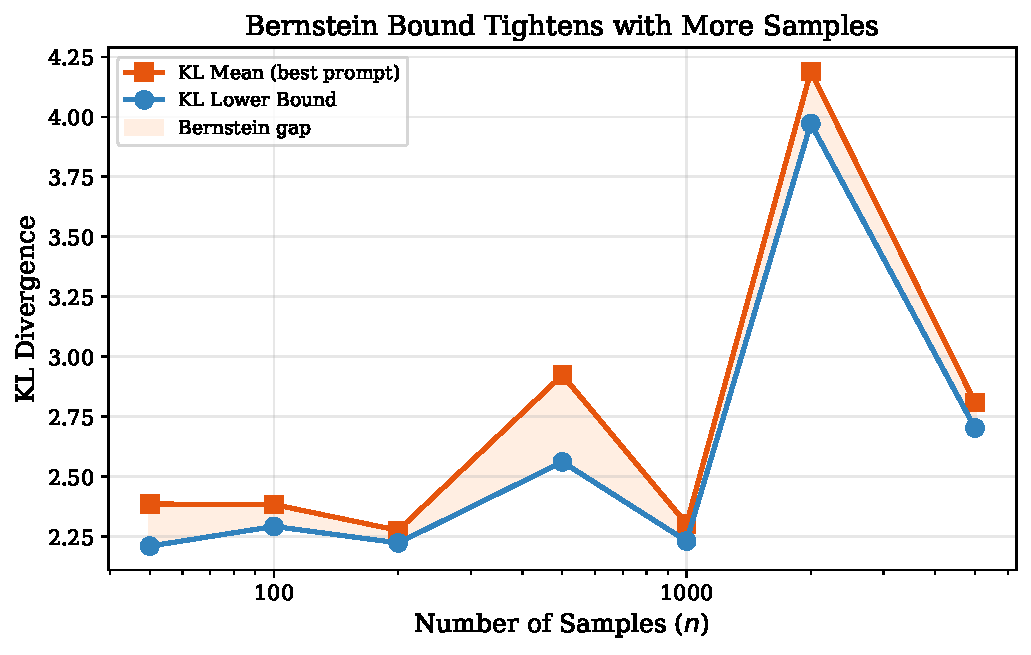
\includegraphics[width=\textwidth]{fig3_sample_ablation.pdf}
\vspace{-6pt}
\centerline{\small (a) Sample-count ablation}
\end{minipage}\hfill
\begin{minipage}[b]{0.48\textwidth}
\centering
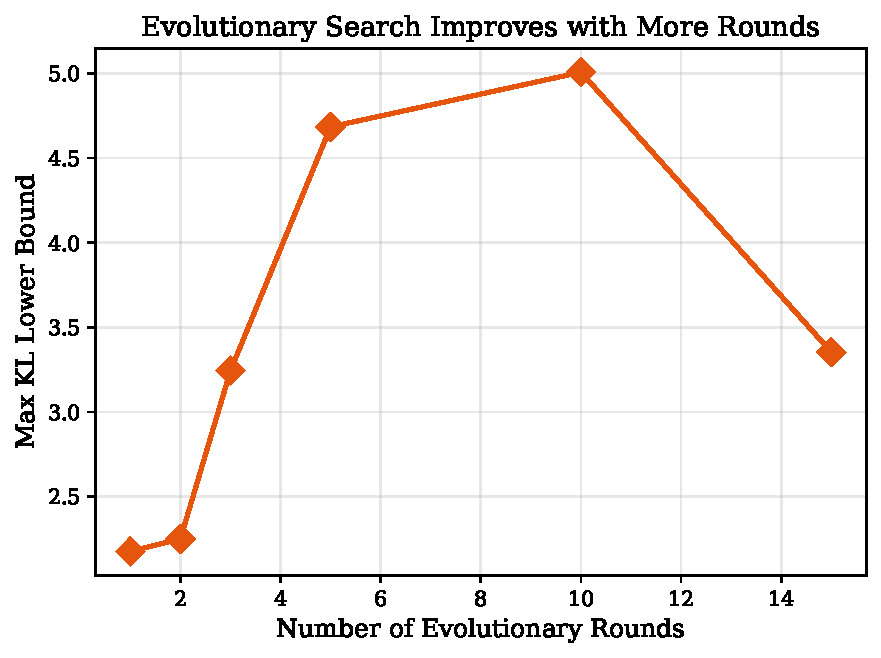
\includegraphics[width=\textwidth]{fig4_round_ablation.pdf}
\vspace{-6pt}
\centerline{\small (b) Round ablation}
\end{minipage}\\[4pt]
\begin{minipage}[b]{0.48\textwidth}
\centering
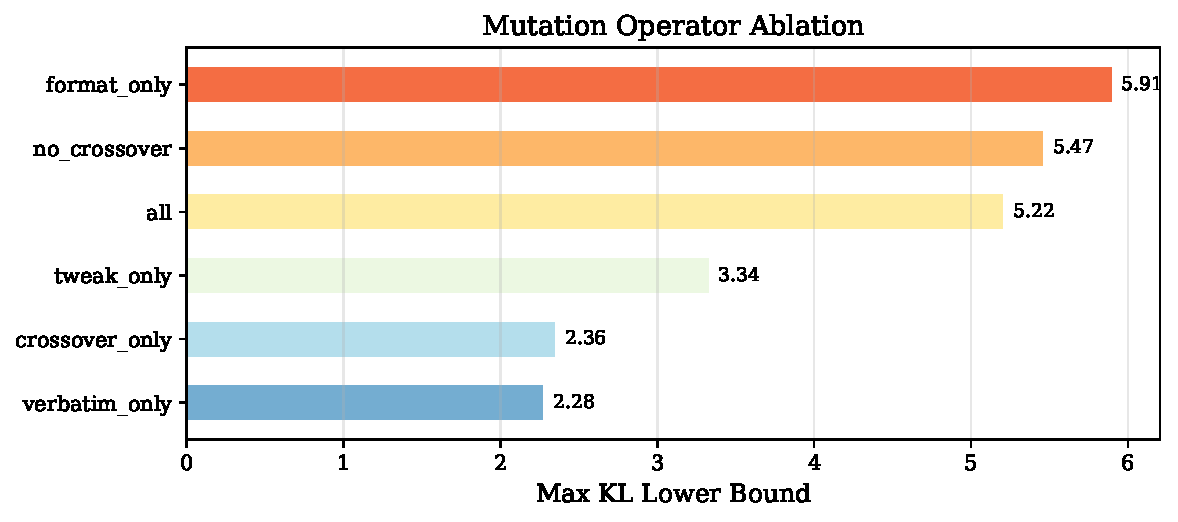
\includegraphics[width=\textwidth]{fig5_mutation_ablation.pdf}
\vspace{-6pt}
\centerline{\small (c) Mutation-operator ablation}
\end{minipage}\hfill
\begin{minipage}[b]{0.48\textwidth}
\centering
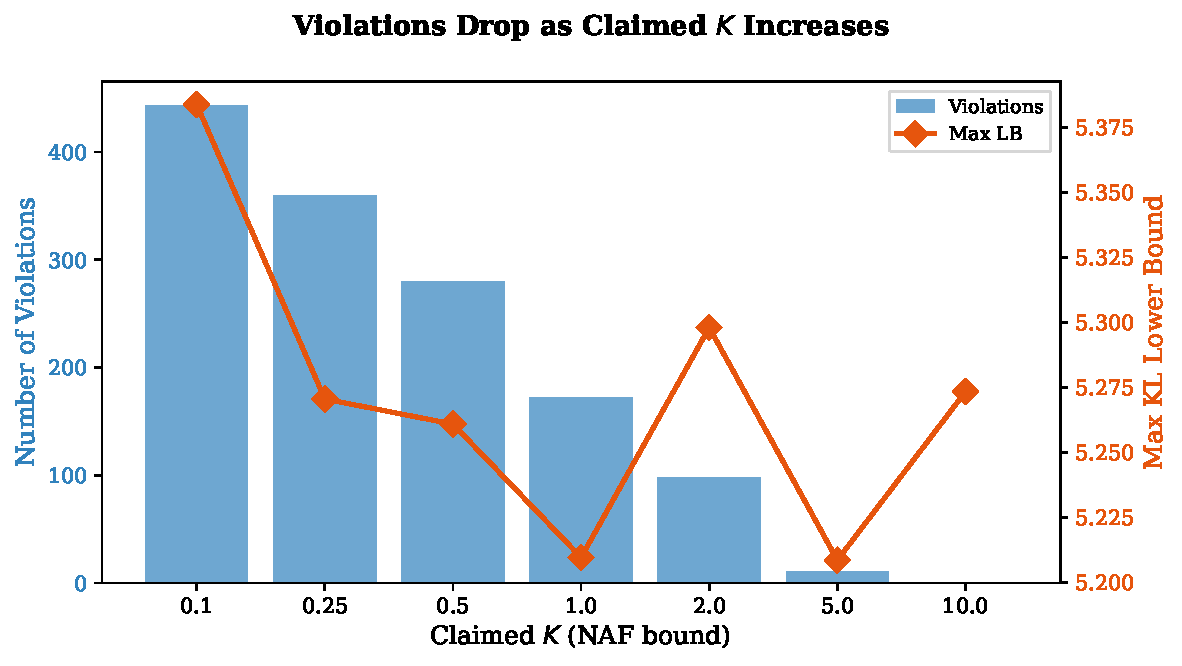
\includegraphics[width=\textwidth]{fig6_k_threshold.pdf}
\vspace{-6pt}
\centerline{\small (d) $K$-threshold sweep}
\end{minipage}
\vspace{-2pt}
\caption{\textbf{Mid-report ablations.}  (a) Bound tightens as $\sqrt n$.  (b) Search improves up to ${\sim}5$ rounds.  (c) Format mutations dominate.  (d) Violations decay as $K$ grows.}
\label{fig:midsem-ablations}
\end{figure}

\begin{figure}[H]
\centering
\begin{minipage}[b]{0.49\textwidth}
\centering
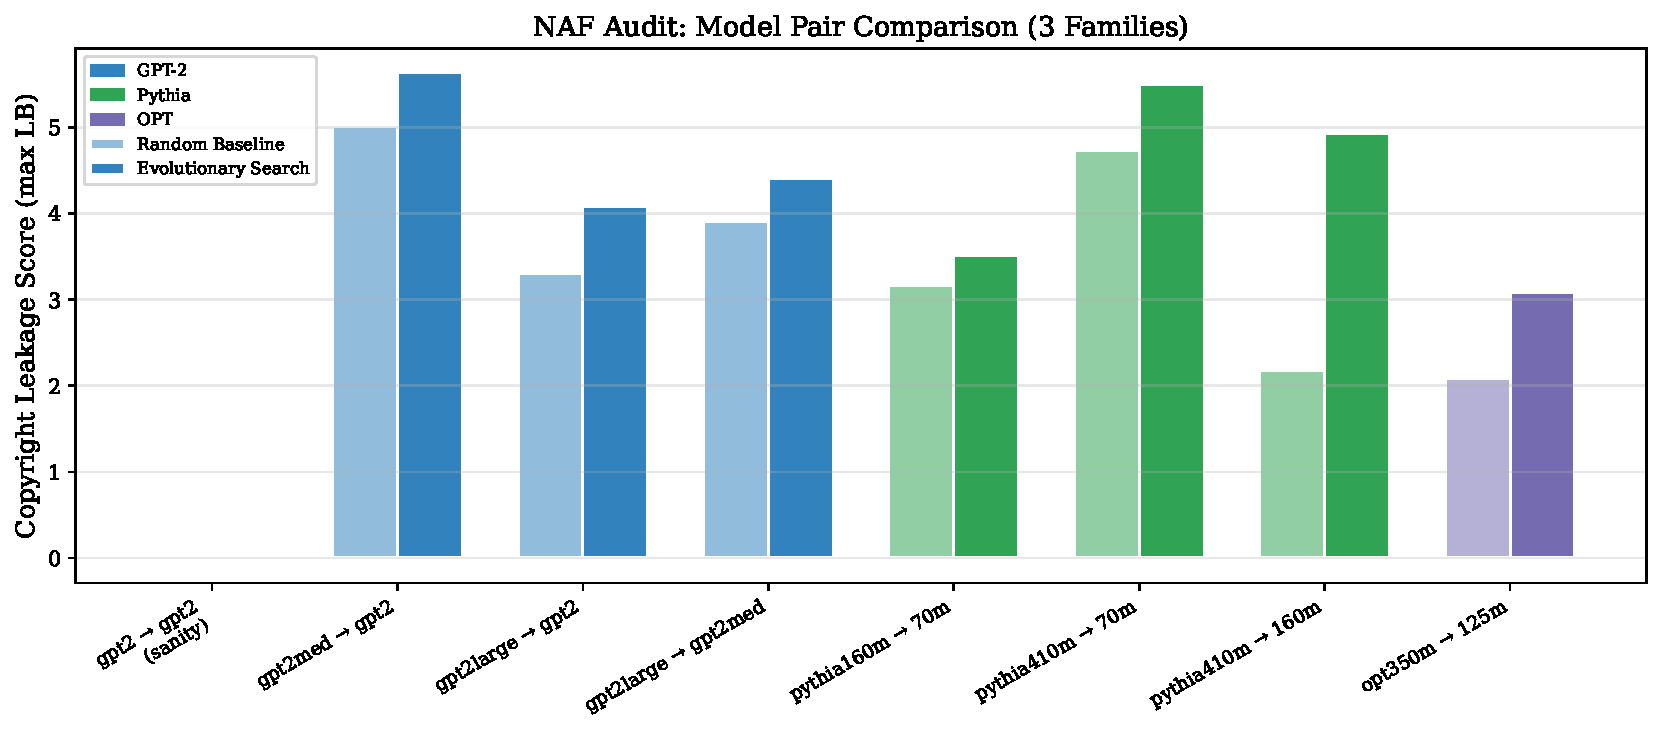
\includegraphics[width=\textwidth]{fig1_model_pairs.pdf}
\vspace{-6pt}
\centerline{\small (a) CLS across eight model pairs}
\end{minipage}\hfill
\begin{minipage}[b]{0.49\textwidth}
\centering
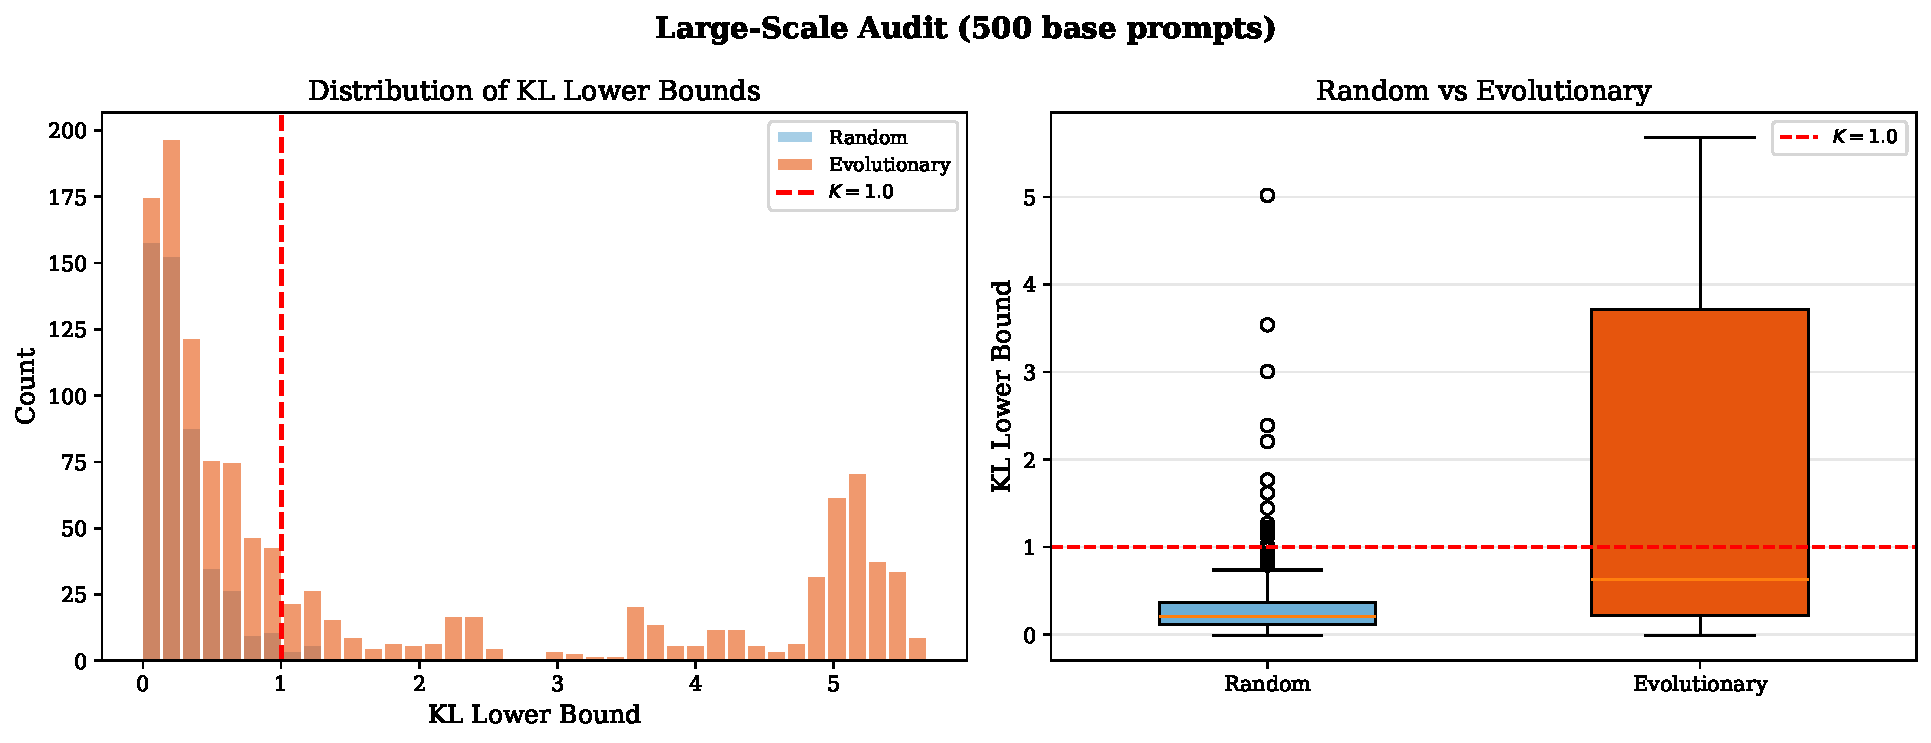
\includegraphics[width=\textwidth]{fig8_largescale.pdf}
\vspace{-6pt}
\centerline{\small (b) Large-scale audit ($500$ prompts)}
\end{minipage}
\vspace{-2pt}
\caption{\textbf{Large-scale and family-wise results.}  (a) Evolutionary search beats random for every non-trivial pair.  (b) $500$ BookMIA prompts $\times\,2000$ samples $\times\,10$ rounds: the search shifts the entire LB distribution up.}
\label{fig:fp1}
\label{fig:fp8}
\end{figure}

\vspace{-4pt}
\begin{figure}[H]
\centering
\begin{minipage}[b]{0.42\textwidth}
\centering
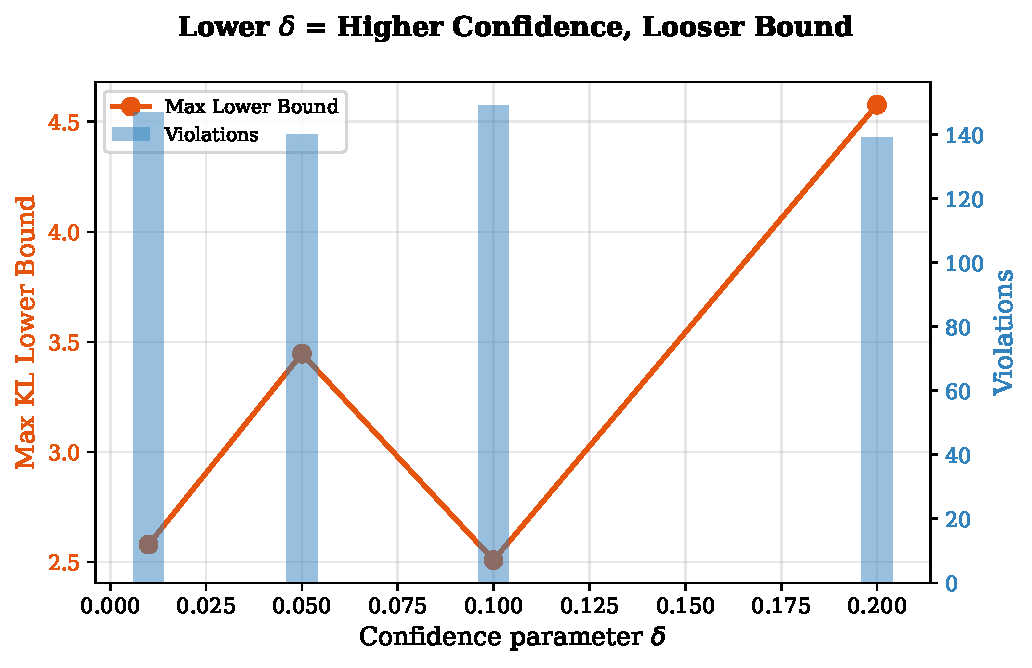
\includegraphics[width=\textwidth]{fig7_delta_sweep.pdf}
\vspace{-6pt}
\centerline{\small (a) $\delta$-sweep}
\end{minipage}\hfill
\begin{minipage}[b]{0.55\textwidth}
\centering
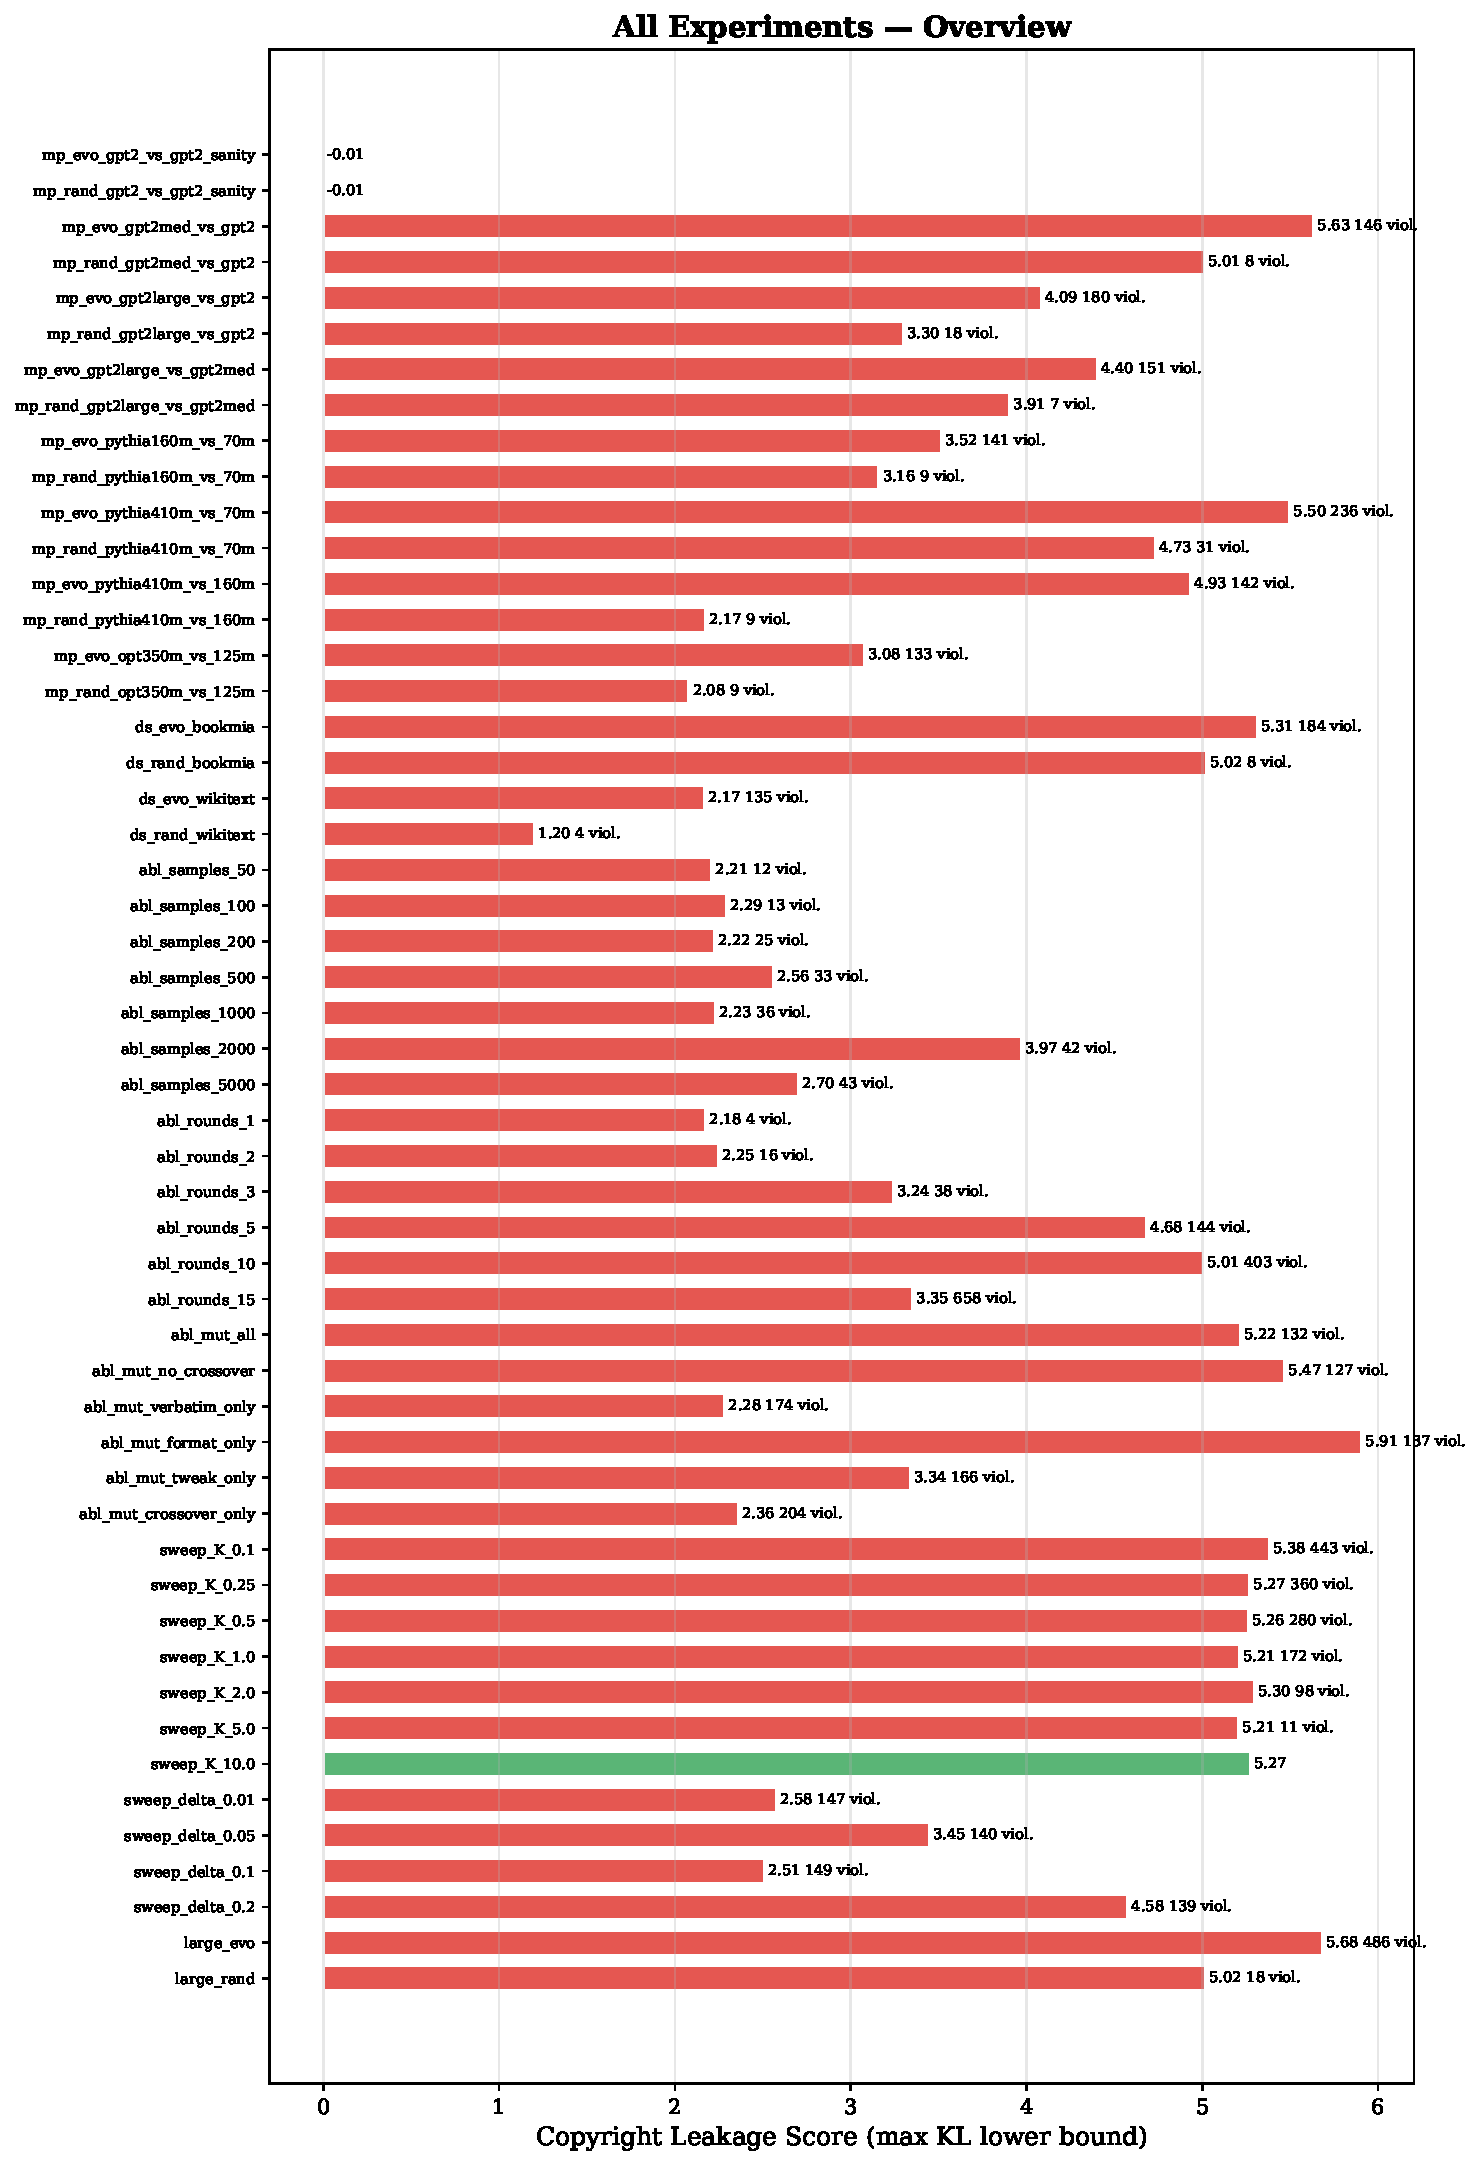
\includegraphics[width=\textwidth]{fig9_summary.pdf}
\vspace{-6pt}
\centerline{\small (b) Per-experiment overview}
\end{minipage}
\vspace{-2pt}
\caption{(a) Tighter $\delta$ produces a (slightly) looser LB, as predicted by the $\ln(2/\delta)$ term.  (b) Bird's-eye view of $52$ sub-experiments; red bars are settings with $\ge 1$ violation.}
\label{fig:fp79}
\end{figure}

\end{document}
